% Be sure to include the Heading Appendix A: before you type the name of the Appendix.
\chapter{Appendix C: Supplemental results}\label{appendix:supplemental-results}

% Appendices should appear at the very end of your thesis. Make sure to label each Appendix with a letter starting with "A". Any tables and/or figures located in the appendix should be labeled accordingly. For example, below is figure A.1 because it is the first figure that appears in Appendix A.

\renewcommand{\thechapter}{C}
\renewcommand{\thefigure}{C.\arabic{figure}}
\setcounter{figure}{0}

\begin{figure}
    \centering
    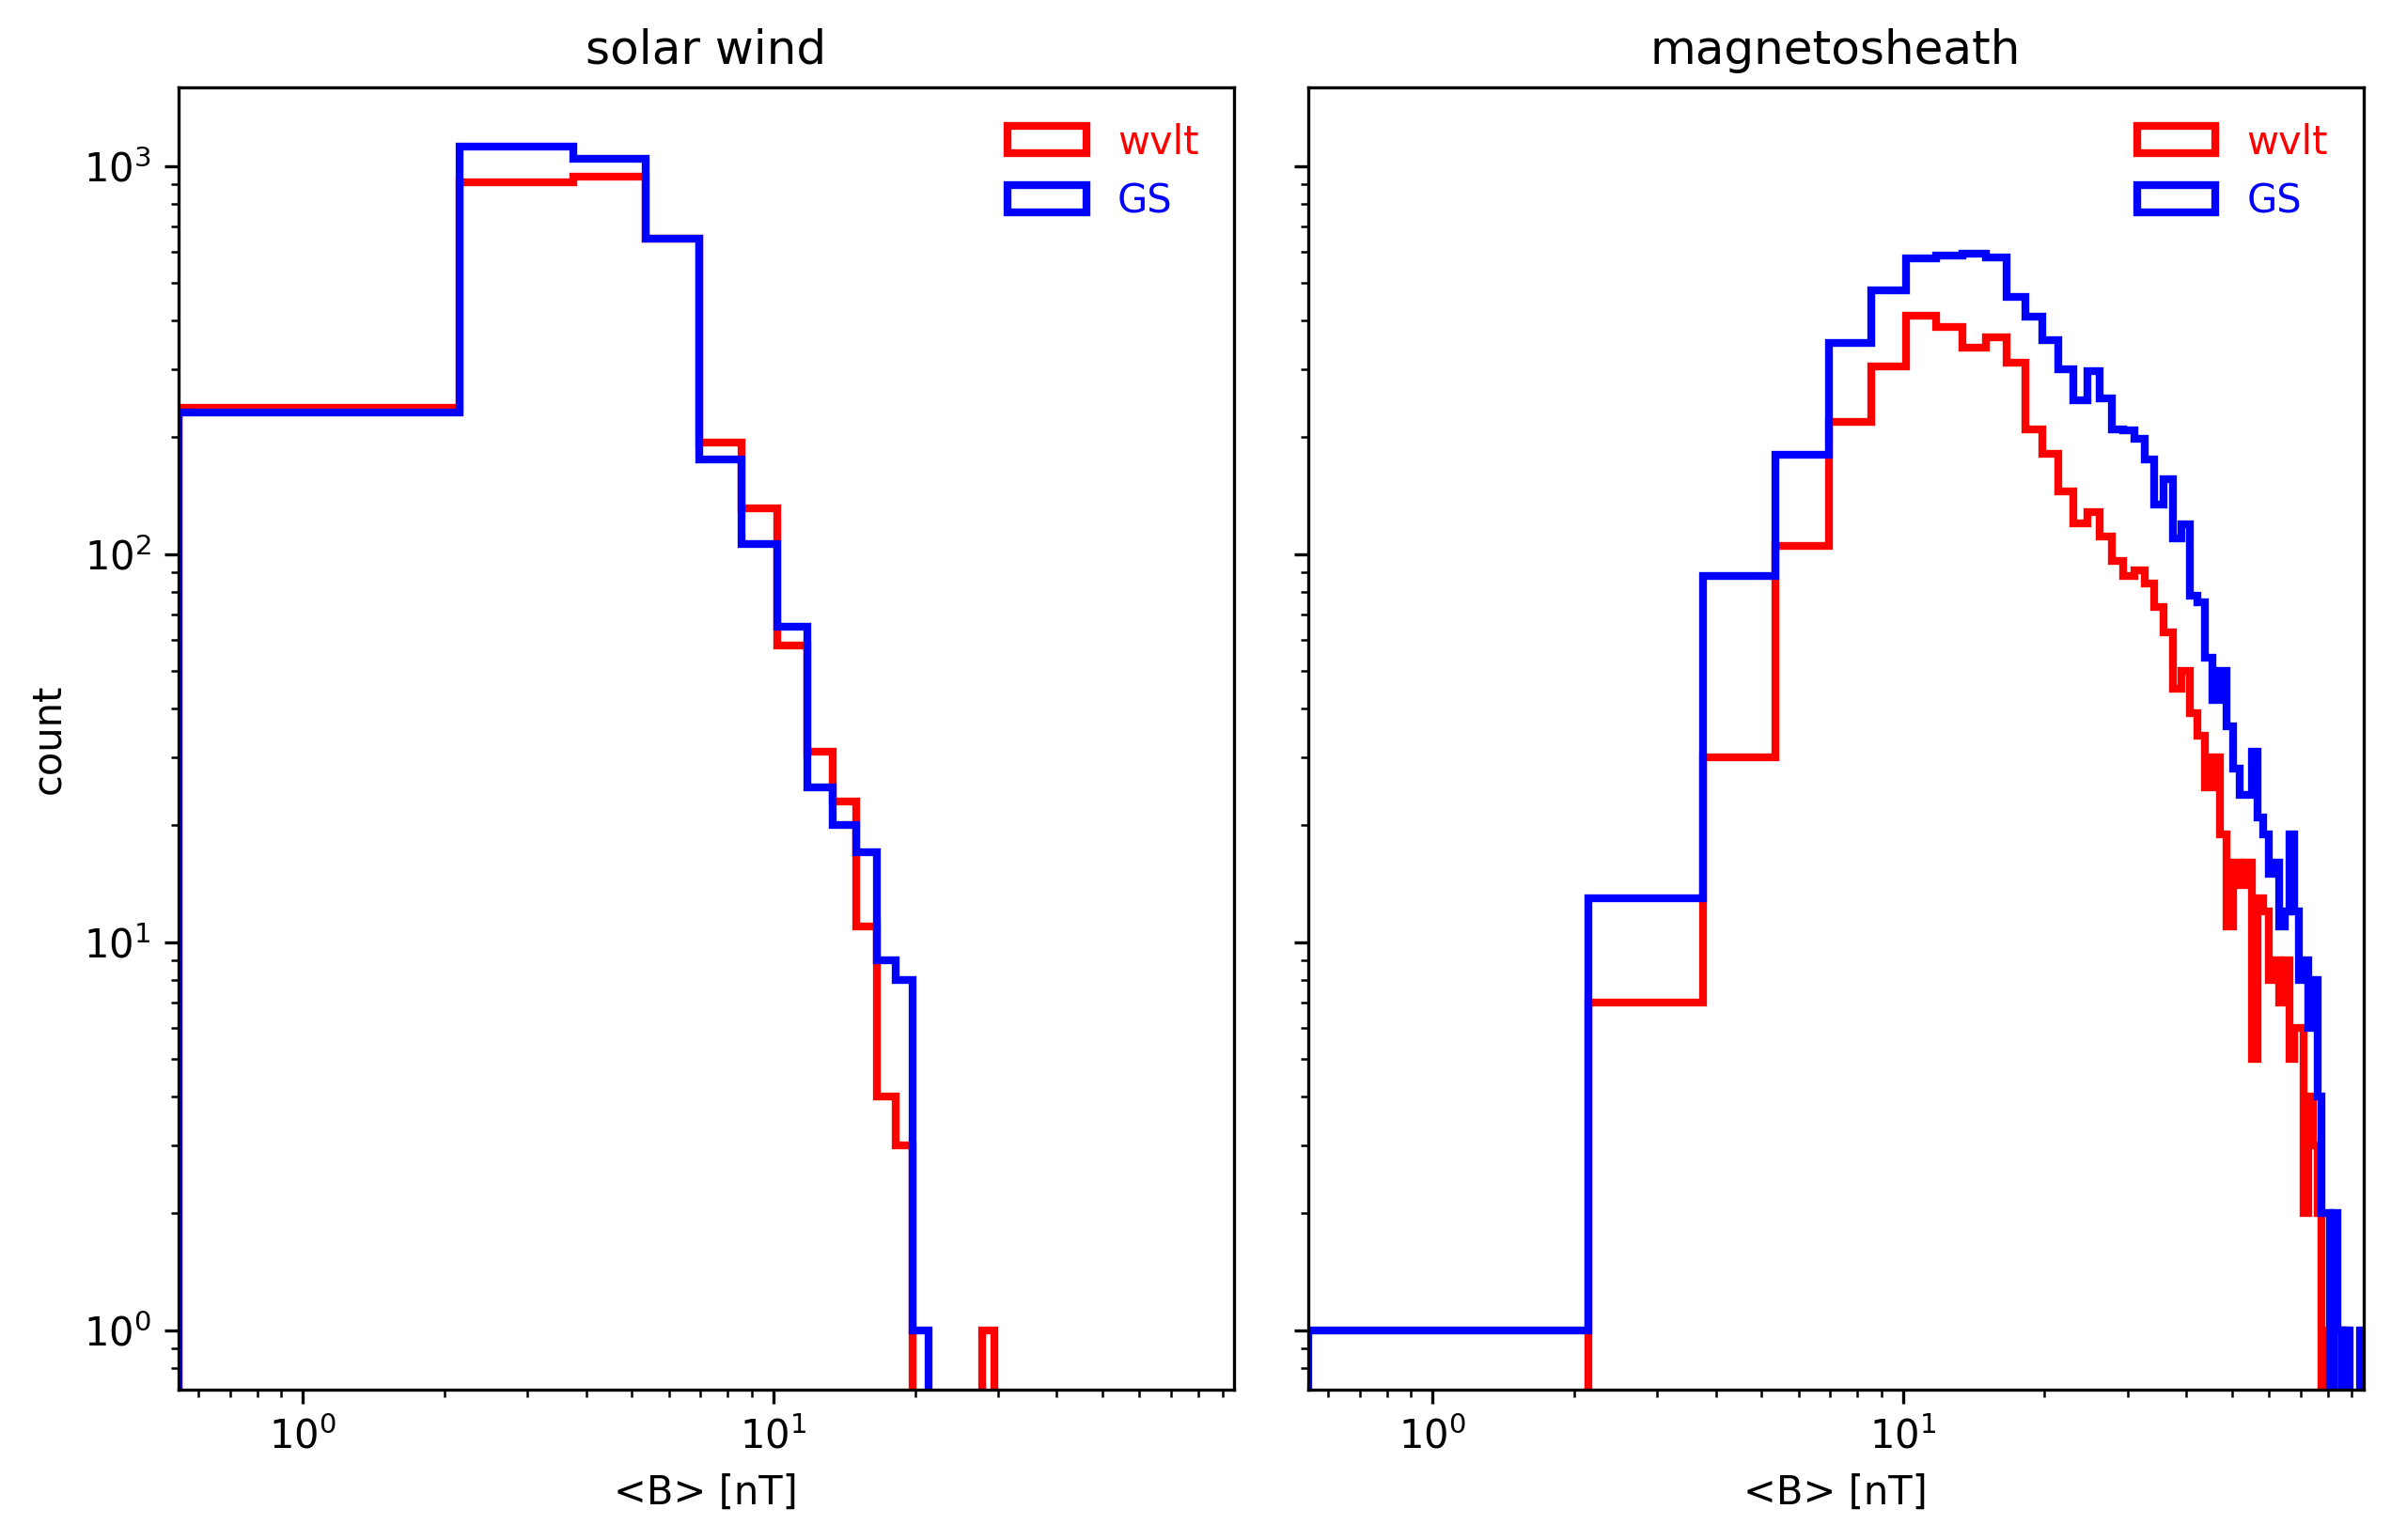
\includegraphics[width=\textwidth]{Figures/Histograms/histogram_Bfield.png}
    \caption[Histogram of average magnetic field for identified events]{Same as Figure \ref{fig:histogram-duration} but for magnetic field distributions of identified events}
    \label{fig:histogram-Bfield}
\end{figure}

\begin{figure}
    \centering
    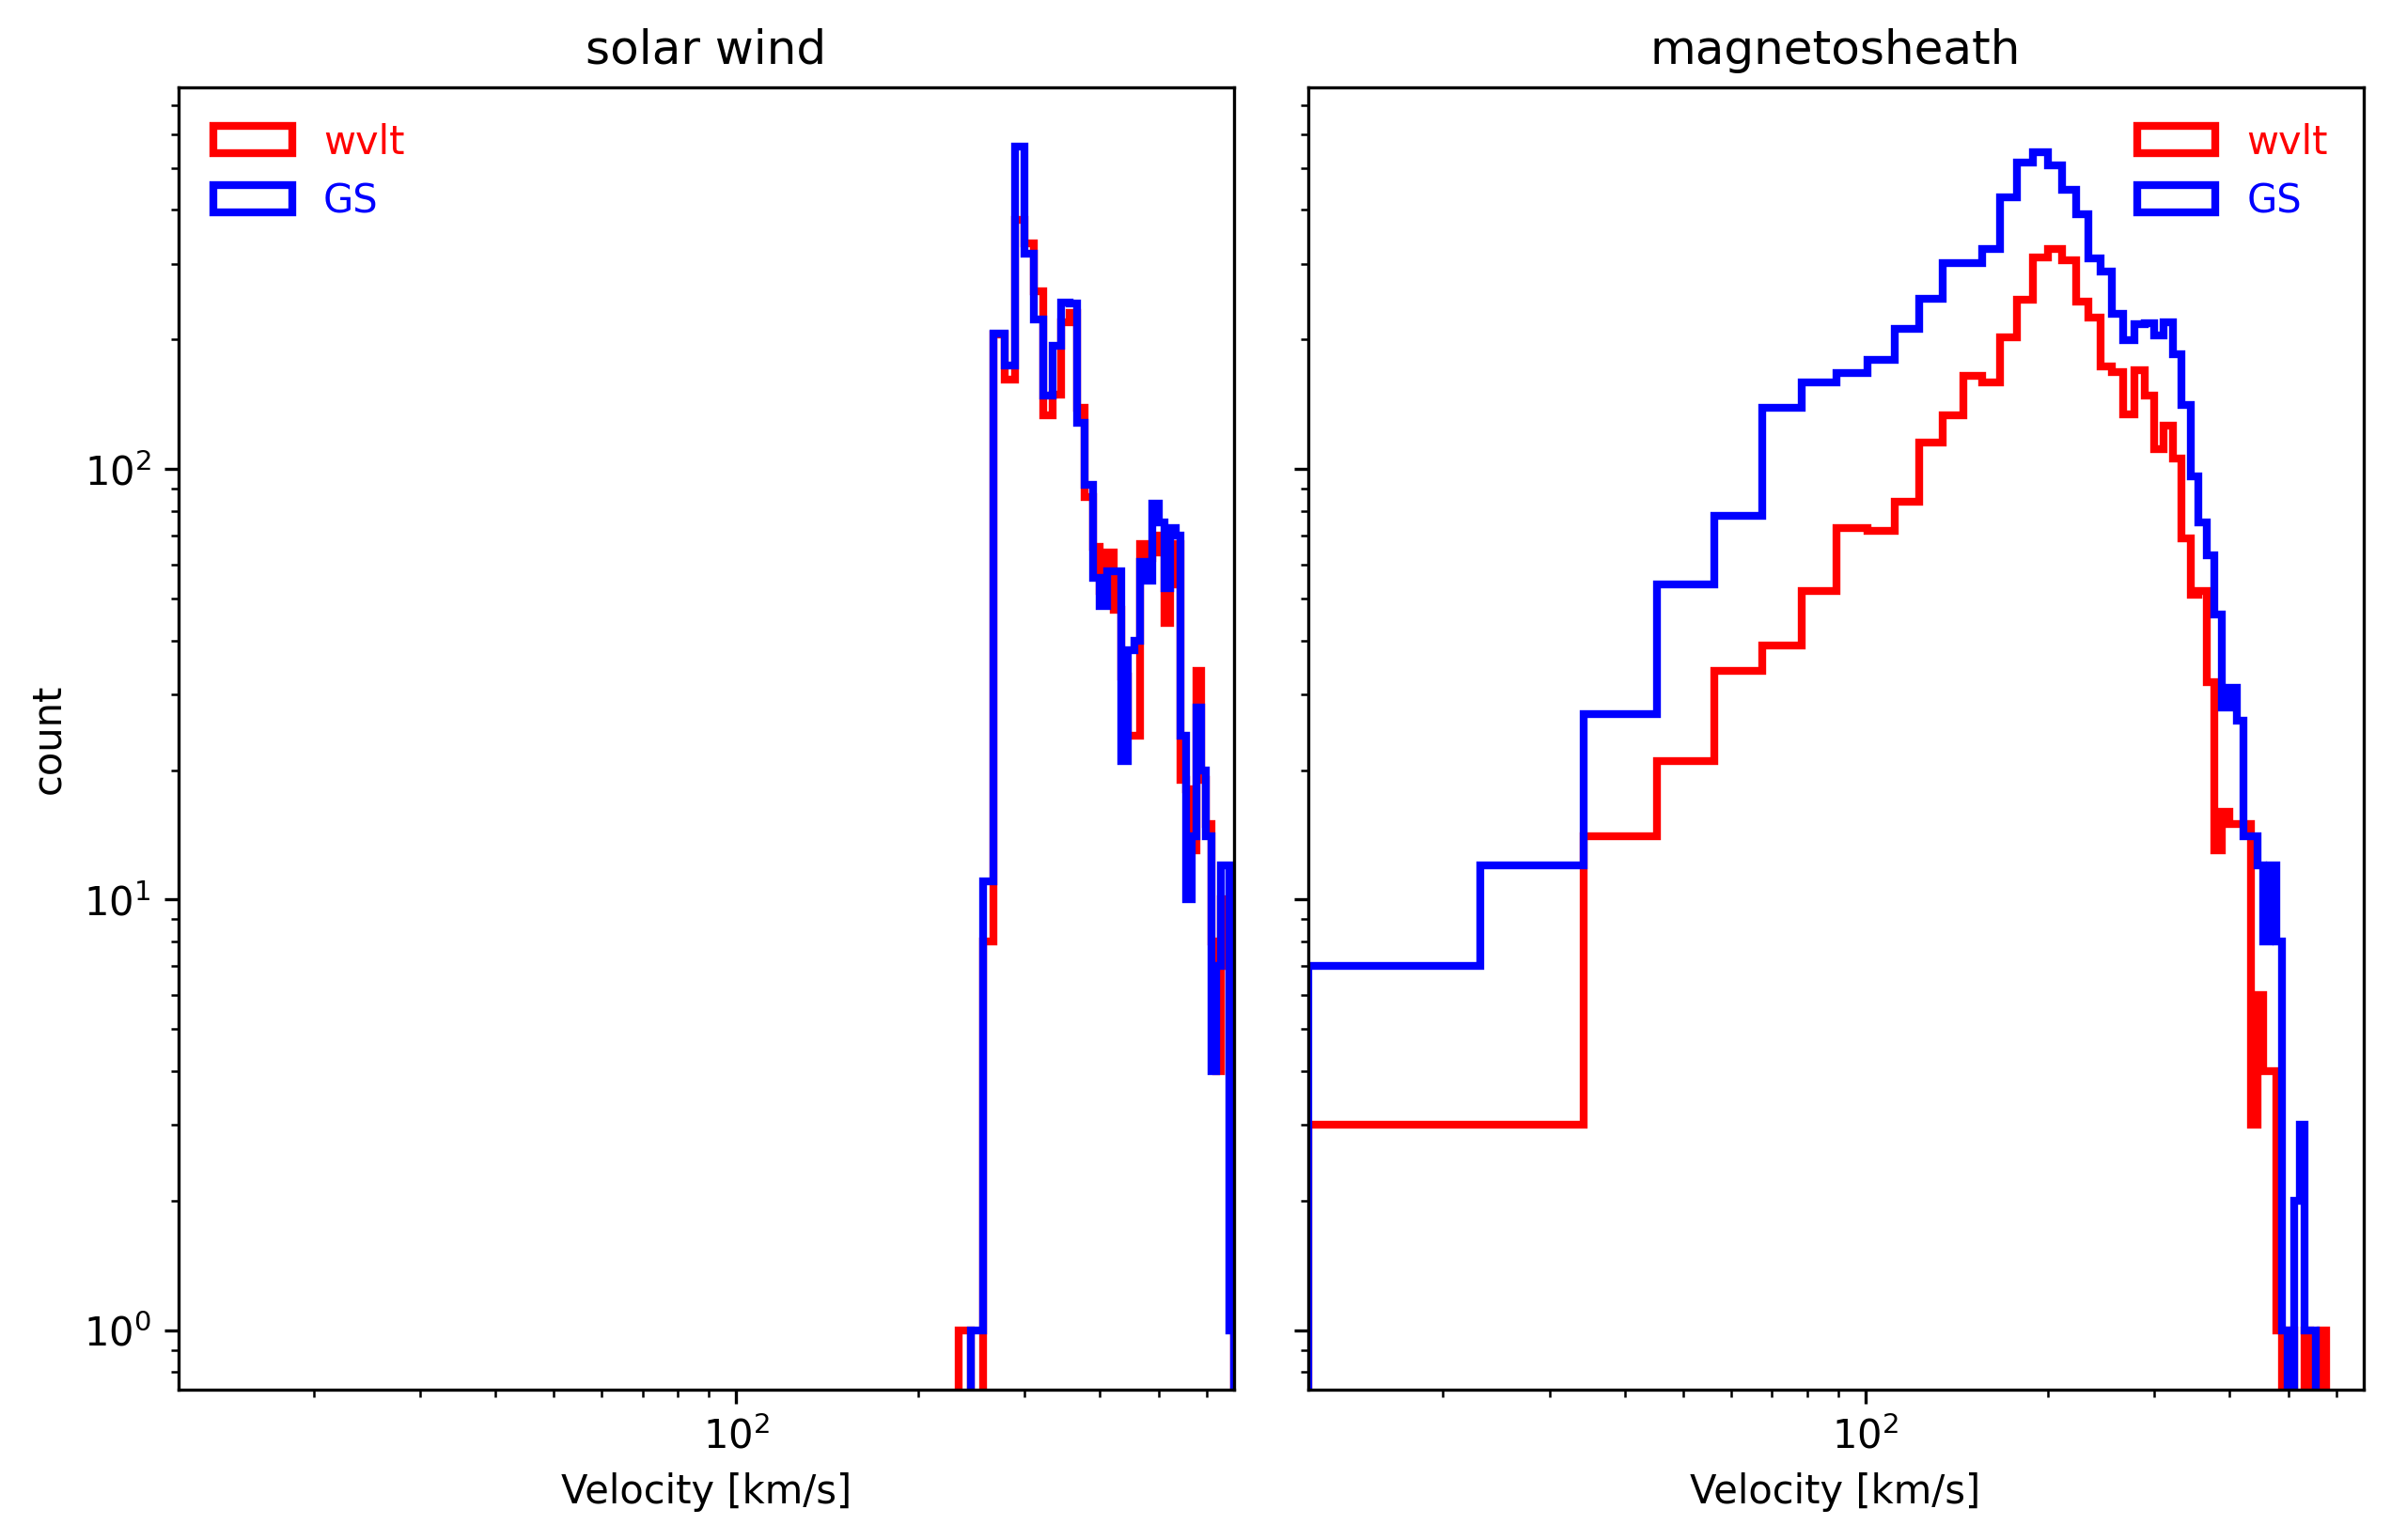
\includegraphics[width=\textwidth]{Figures/Histograms/histogram_velocity.png}
    \caption[Histogram of velocity for identified events]{Same as Figure \ref{fig:histogram-duration} but for velocity distributions of identified events}
    \label{fig:histogram-velocity}
\end{figure}

\begin{figure}
    \centering
    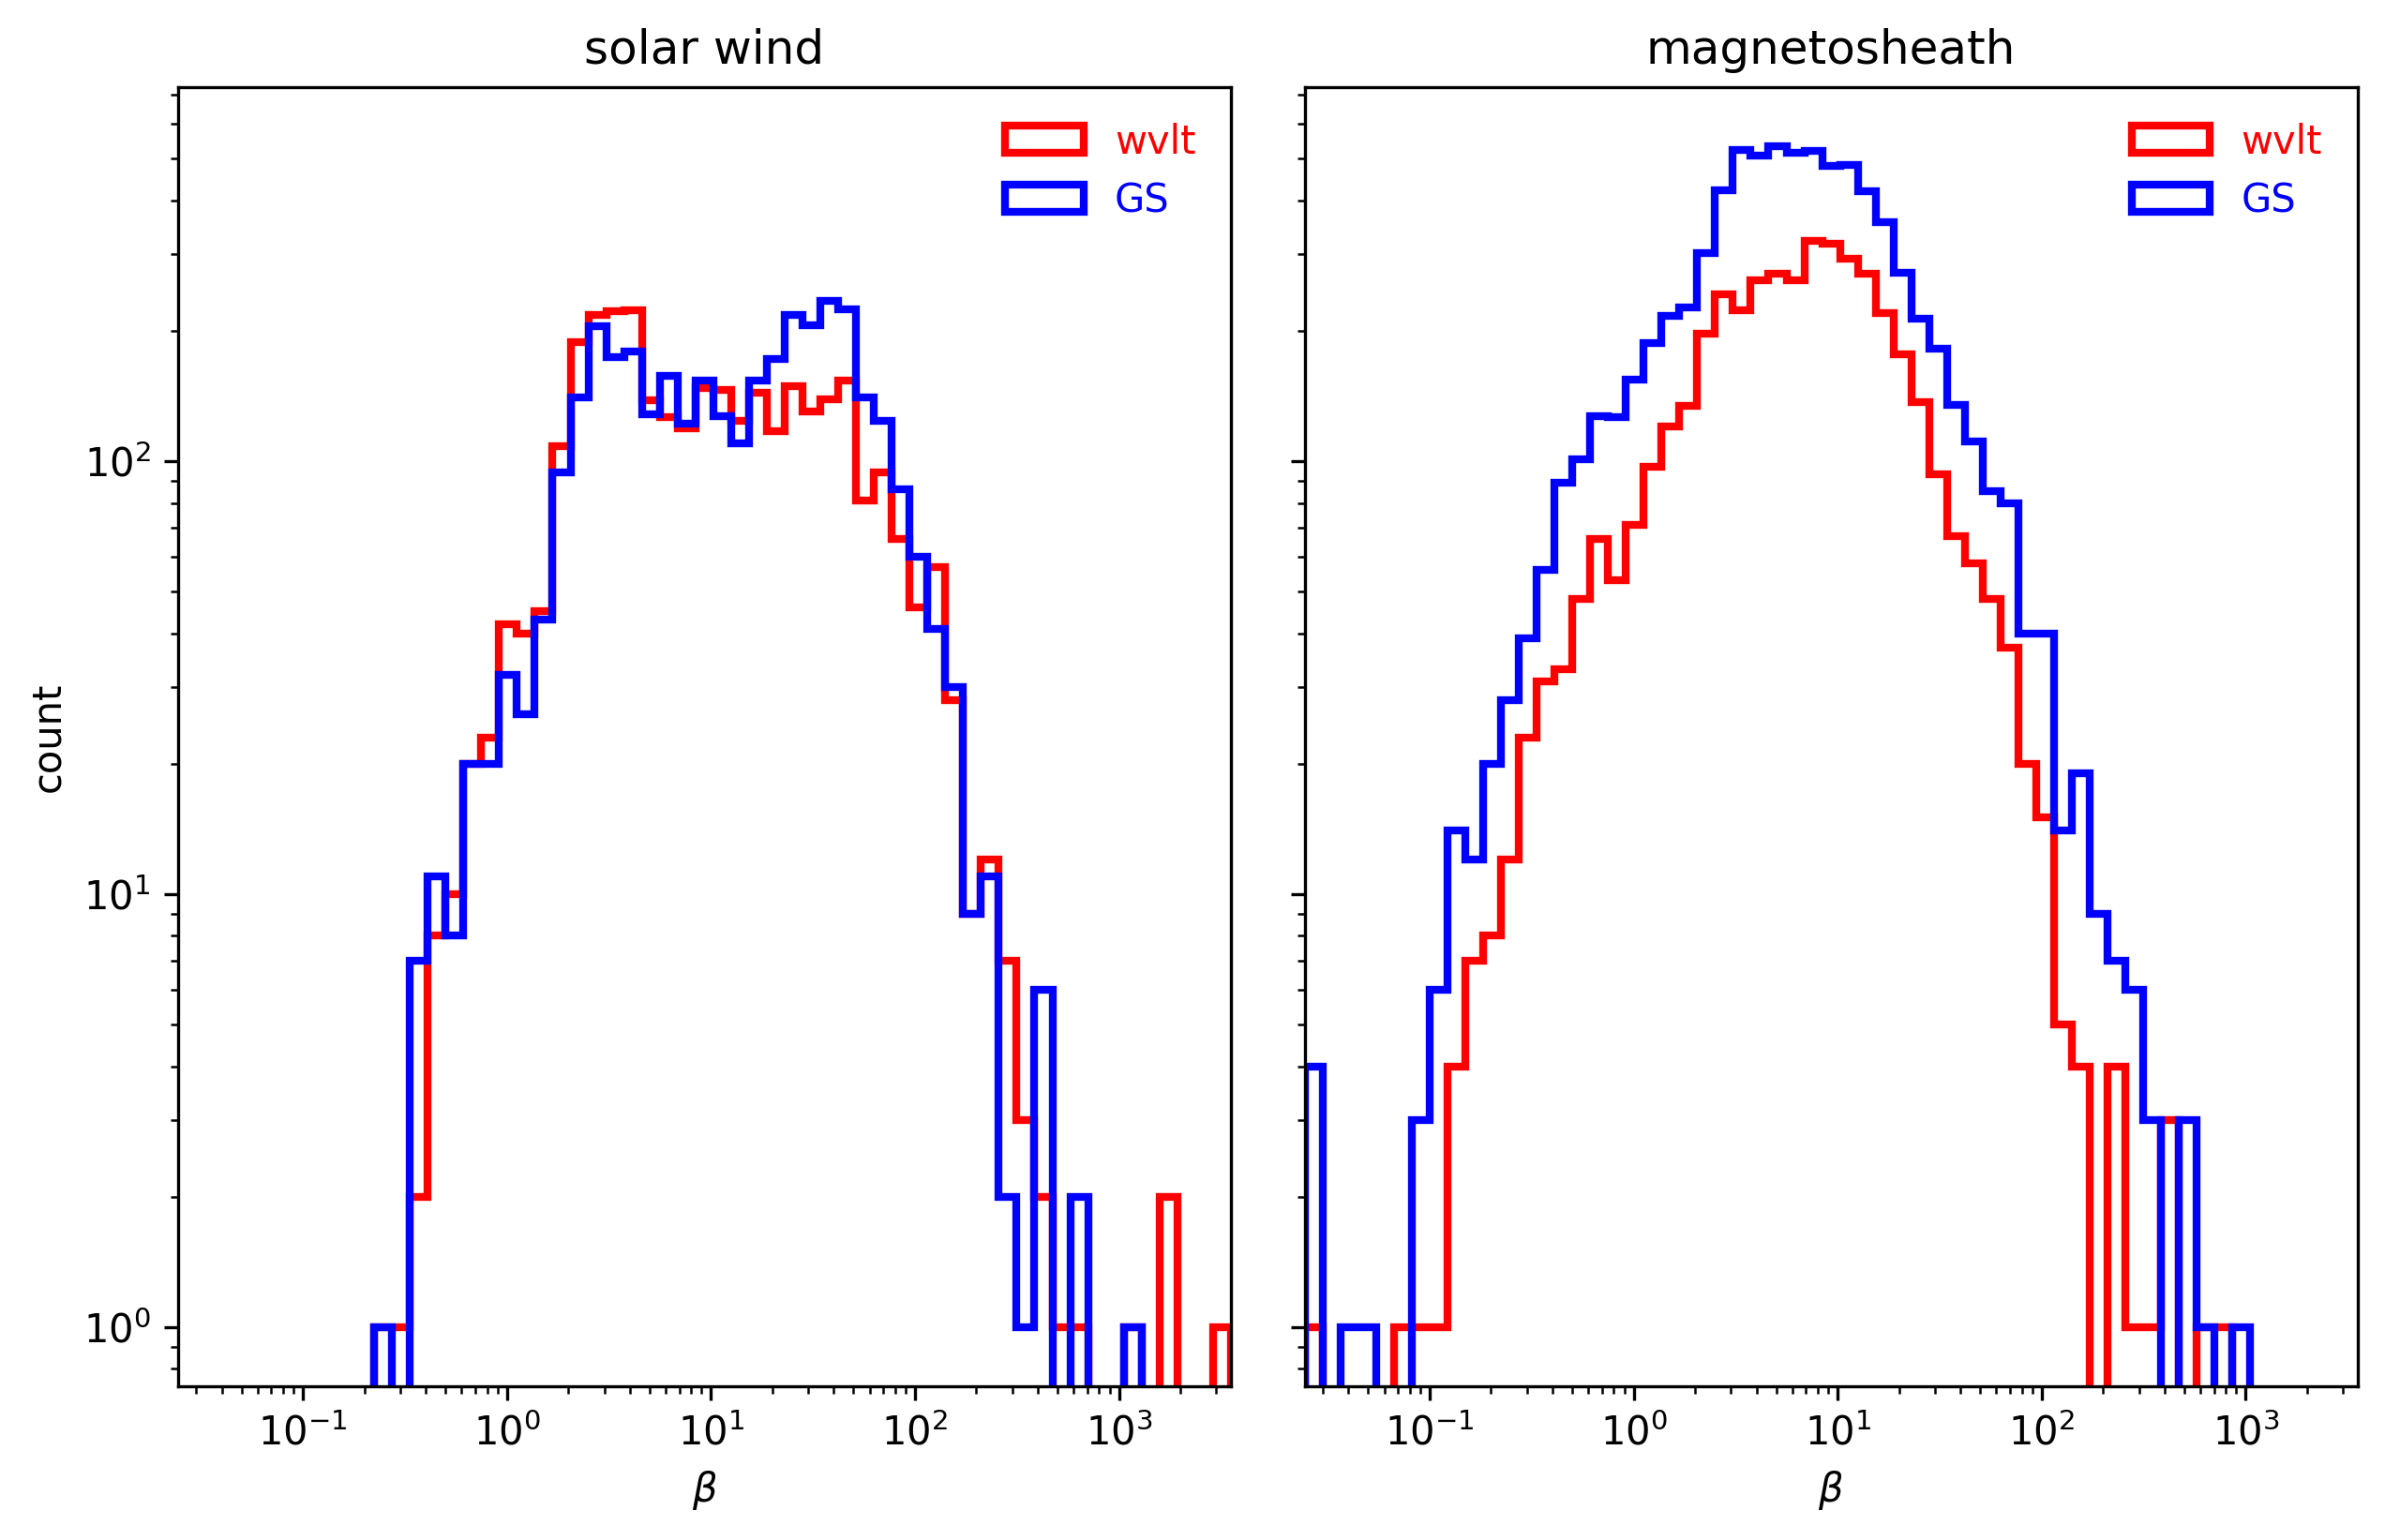
\includegraphics[width=\textwidth]{Figures/Histograms/histogram_logspace_beta.png}
    \caption[Histogram of beta for identified events]{Same as Figure \ref{fig:histogram-duration} but for plasma $\beta$ distributions of identified events}
    \label{fig:histogram-beta}
\end{figure}

\begin{figure}
    \centering
    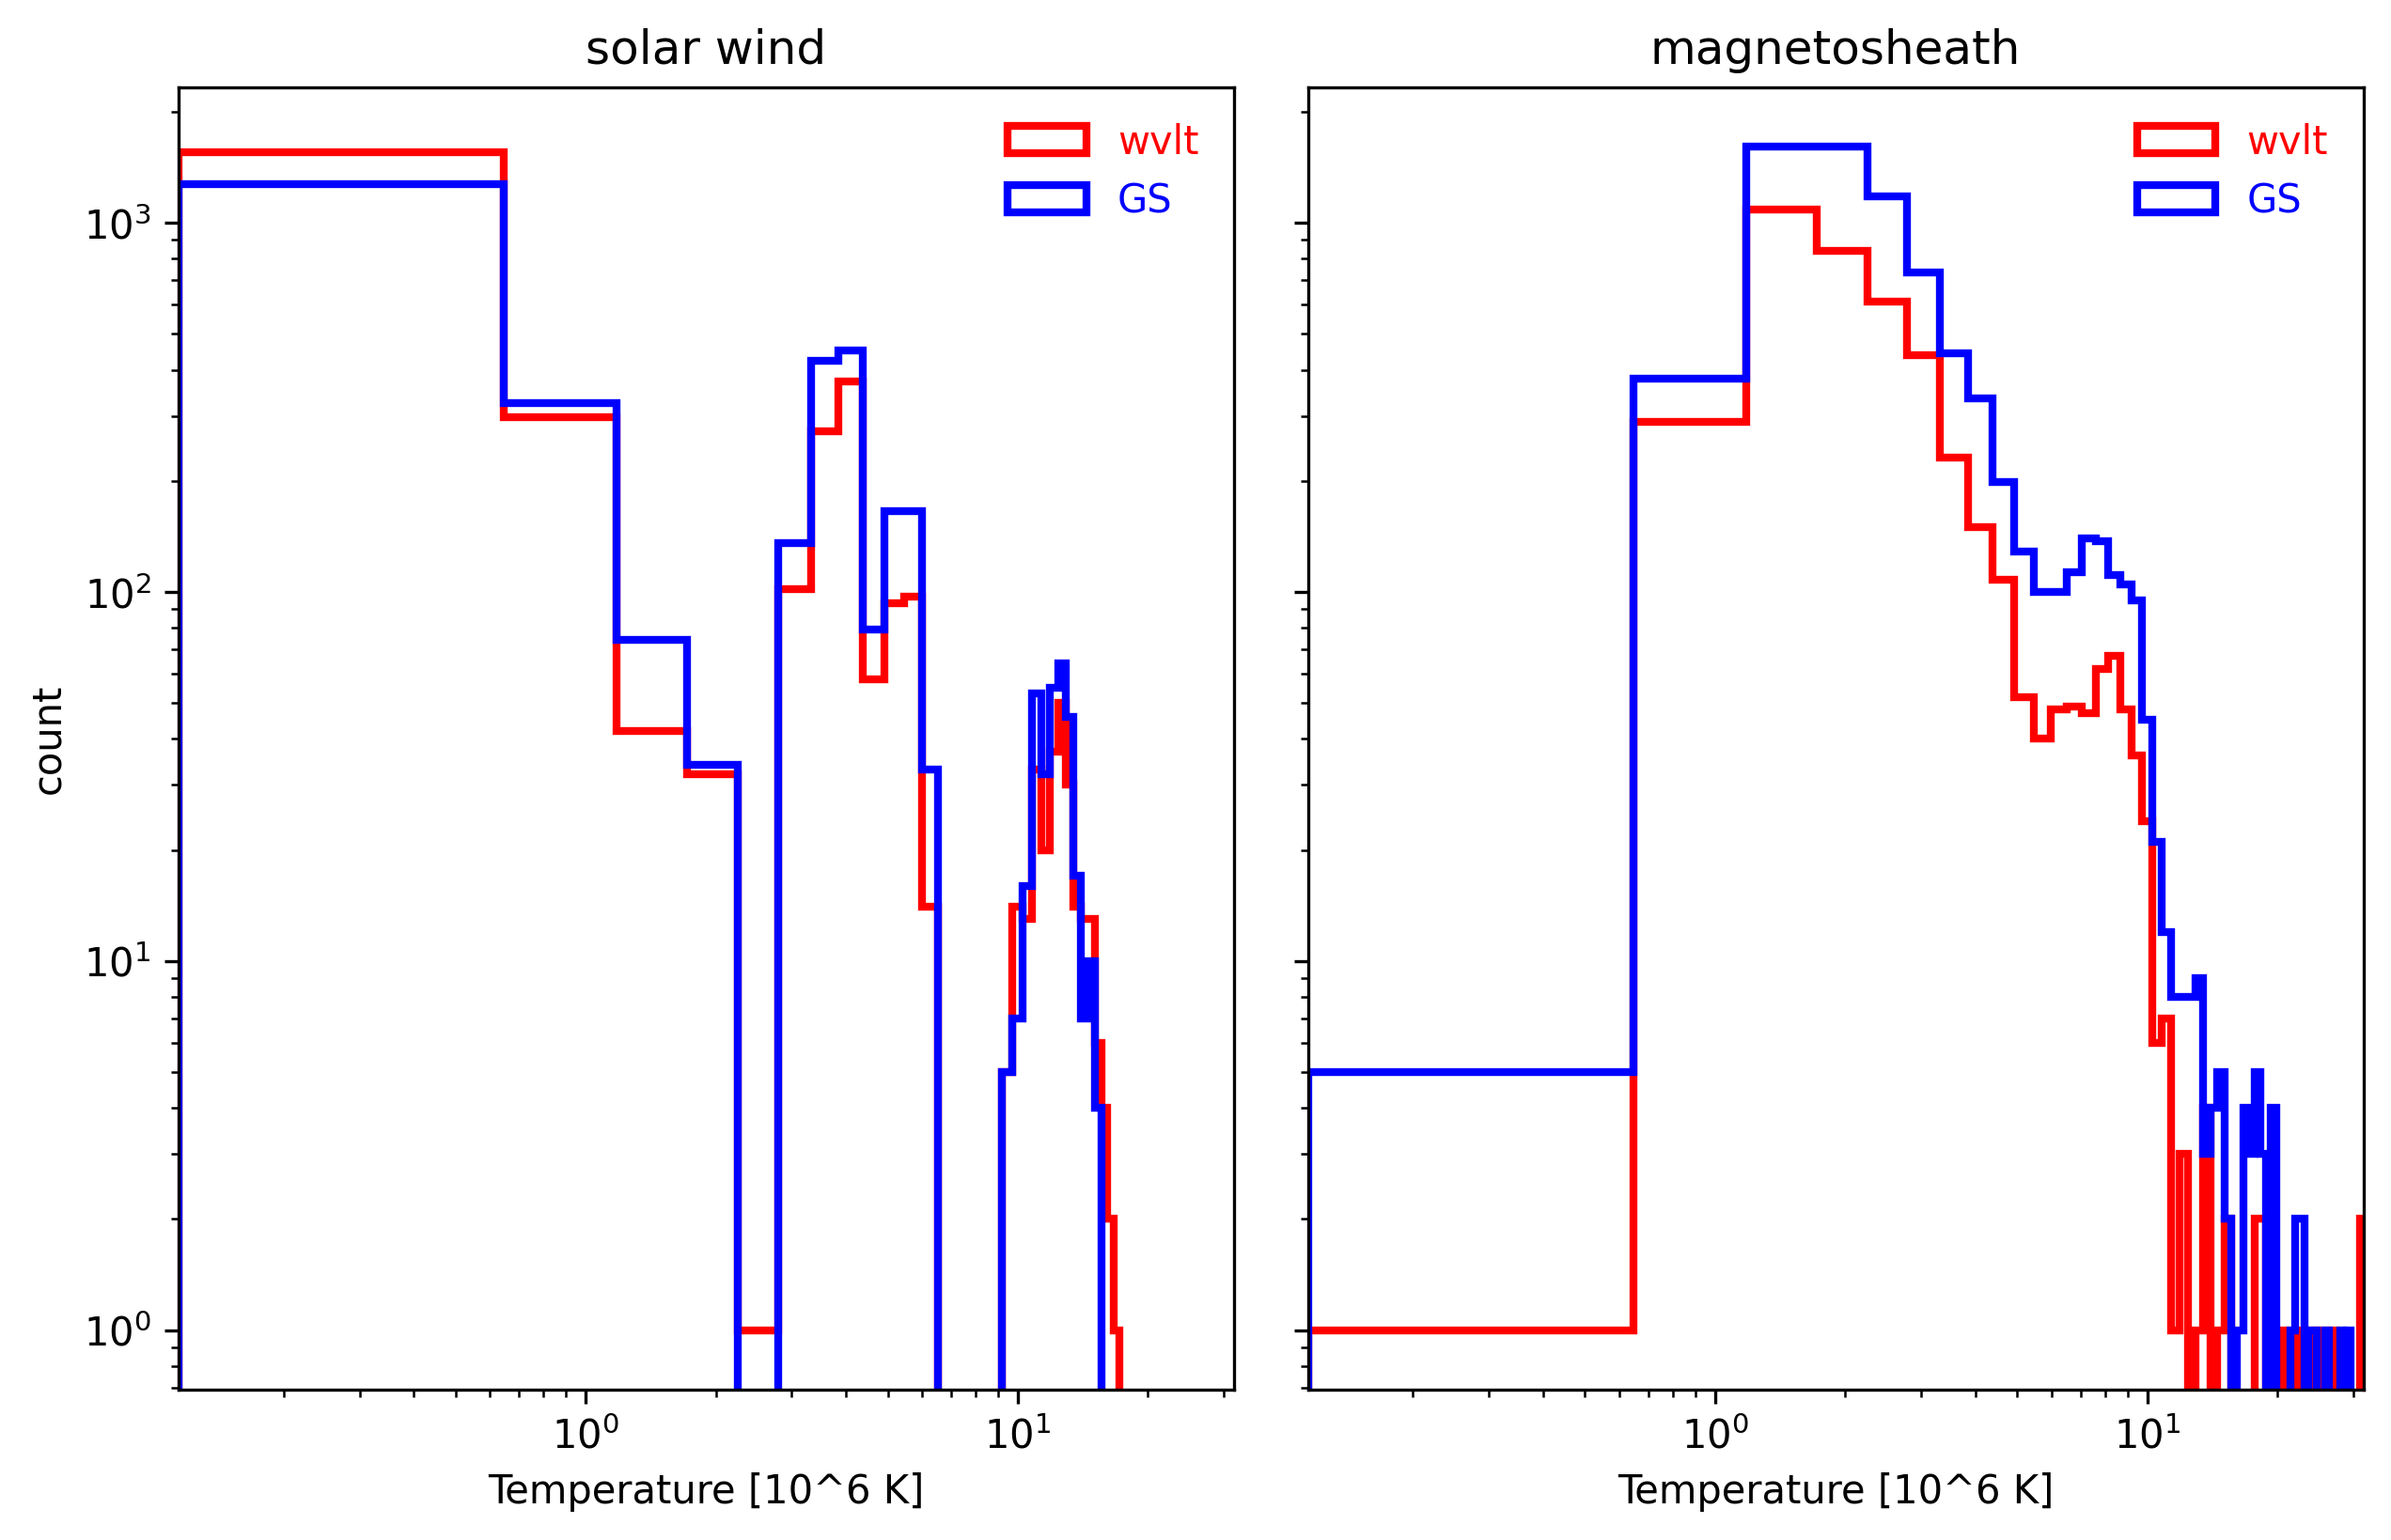
\includegraphics[width=\textwidth]{Figures/Histograms/histogram_temperature.png}
    \caption[Histogram of temperature for identified events]{Same as Figure \ref{fig:histogram-duration} but for temperature distributions of identified events}
    \label{fig:histogram-temp}
\end{figure}